% GNUPLOT: LaTeX picture with Postscript
\begingroup
  \fontfamily{phv}%
  \selectfont
  \makeatletter
  \providecommand\color[2][]{%
    \GenericError{(gnuplot) \space\space\space\@spaces}{%
      Package color not loaded in conjunction with
      terminal option `colourtext'%
    }{See the gnuplot documentation for explanation.%
    }{Either use 'blacktext' in gnuplot or load the package
      color.sty in LaTeX.}%
    \renewcommand\color[2][]{}%
  }%
  \providecommand\includegraphics[2][]{%
    \GenericError{(gnuplot) \space\space\space\@spaces}{%
      Package graphicx or graphics not loaded%
    }{See the gnuplot documentation for explanation.%
    }{The gnuplot epslatex terminal needs graphicx.sty or graphics.sty.}%
    \renewcommand\includegraphics[2][]{}%
  }%
  \providecommand\rotatebox[2]{#2}%
  \@ifundefined{ifGPcolor}{%
    \newif\ifGPcolor
    \GPcolorfalse
  }{}%
  \@ifundefined{ifGPblacktext}{%
    \newif\ifGPblacktext
    \GPblacktexttrue
  }{}%
  % define a \g@addto@macro without @ in the name:
  \let\gplgaddtomacro\g@addto@macro
  % define empty templates for all commands taking text:
  \gdef\gplbacktext{}%
  \gdef\gplfronttext{}%
  \makeatother
  \ifGPblacktext
    % no textcolor at all
    \def\colorrgb#1{}%
    \def\colorgray#1{}%
  \else
    % gray or color?
    \ifGPcolor
      \def\colorrgb#1{\color[rgb]{#1}}%
      \def\colorgray#1{\color[gray]{#1}}%
      \expandafter\def\csname LTw\endcsname{\color{white}}%
      \expandafter\def\csname LTb\endcsname{\color{black}}%
      \expandafter\def\csname LTa\endcsname{\color{black}}%
      \expandafter\def\csname LT0\endcsname{\color[rgb]{1,0,0}}%
      \expandafter\def\csname LT1\endcsname{\color[rgb]{0,1,0}}%
      \expandafter\def\csname LT2\endcsname{\color[rgb]{0,0,1}}%
      \expandafter\def\csname LT3\endcsname{\color[rgb]{1,0,1}}%
      \expandafter\def\csname LT4\endcsname{\color[rgb]{0,1,1}}%
      \expandafter\def\csname LT5\endcsname{\color[rgb]{1,1,0}}%
      \expandafter\def\csname LT6\endcsname{\color[rgb]{0,0,0}}%
      \expandafter\def\csname LT7\endcsname{\color[rgb]{1,0.3,0}}%
      \expandafter\def\csname LT8\endcsname{\color[rgb]{0.5,0.5,0.5}}%
    \else
      % gray
      \def\colorrgb#1{\color{black}}%
      \def\colorgray#1{\color[gray]{#1}}%
      \expandafter\def\csname LTw\endcsname{\color{white}}%
      \expandafter\def\csname LTb\endcsname{\color{black}}%
      \expandafter\def\csname LTa\endcsname{\color{black}}%
      \expandafter\def\csname LT0\endcsname{\color{black}}%
      \expandafter\def\csname LT1\endcsname{\color{black}}%
      \expandafter\def\csname LT2\endcsname{\color{black}}%
      \expandafter\def\csname LT3\endcsname{\color{black}}%
      \expandafter\def\csname LT4\endcsname{\color{black}}%
      \expandafter\def\csname LT5\endcsname{\color{black}}%
      \expandafter\def\csname LT6\endcsname{\color{black}}%
      \expandafter\def\csname LT7\endcsname{\color{black}}%
      \expandafter\def\csname LT8\endcsname{\color{black}}%
    \fi
  \fi
    \setlength{\unitlength}{0.0500bp}%
    \ifx\gptboxheight\undefined%
      \newlength{\gptboxheight}%
      \newlength{\gptboxwidth}%
      \newsavebox{\gptboxtext}%
    \fi%
    \setlength{\fboxrule}{0.5pt}%
    \setlength{\fboxsep}{1pt}%
\begin{picture}(7200.00,5040.00)%
    \gplgaddtomacro\gplbacktext{%
      \csname LTb\endcsname%
      \put(858,704){\makebox(0,0)[r]{\strut{}\footnotesize -10}}%
      \put(858,1072){\makebox(0,0)[r]{\strut{}\footnotesize -9}}%
      \put(858,1439){\makebox(0,0)[r]{\strut{}\footnotesize -8}}%
      \put(858,1807){\makebox(0,0)[r]{\strut{}\footnotesize -7}}%
      \put(858,2174){\makebox(0,0)[r]{\strut{}\footnotesize -6}}%
      \put(858,2542){\makebox(0,0)[r]{\strut{}\footnotesize -5}}%
      \put(858,2909){\makebox(0,0)[r]{\strut{}\footnotesize -4}}%
      \put(858,3277){\makebox(0,0)[r]{\strut{}\footnotesize -3}}%
      \put(858,3644){\makebox(0,0)[r]{\strut{}\footnotesize -2}}%
      \put(858,4012){\makebox(0,0)[r]{\strut{}\footnotesize -1}}%
      \put(858,4379){\makebox(0,0)[r]{\strut{}\footnotesize 0}}%
      \put(1571,484){\makebox(0,0){\strut{}\footnotesize 100}}%
      \put(2153,484){\makebox(0,0){\strut{}\footnotesize 200}}%
      \put(2734,484){\makebox(0,0){\strut{}\footnotesize 300}}%
      \put(3315,484){\makebox(0,0){\strut{}\footnotesize 400}}%
      \put(3897,484){\makebox(0,0){\strut{}\footnotesize 500}}%
      \put(4478,484){\makebox(0,0){\strut{}\footnotesize 600}}%
      \put(5059,484){\makebox(0,0){\strut{}\footnotesize 700}}%
      \put(5640,484){\makebox(0,0){\strut{}\footnotesize 800}}%
      \put(6222,484){\makebox(0,0){\strut{}\footnotesize 900}}%
    }%
    \gplgaddtomacro\gplfronttext{%
      \csname LTb\endcsname%
      \put(352,2541){\rotatebox{-270}{\makebox(0,0){\strut{}\footnotesize Residual 2-norm, log scale}}}%
      \put(3896,154){\makebox(0,0){\strut{}\footnotesize Iteration count}}%
      \put(3896,4709){\makebox(0,0){\strut{}\shortstack{\footnotesize\,1e+04\,times,1e+04\,diagonal,\,logspace\,eigs,\,cond\,1e+10\\\footnotesize\,Residual\,2-norm,\,log\,scale}}}%
      \csname LTb\endcsname%
      \put(1811,2349){\makebox(0,0)[l]{\strut{}\scriptsize GMRES(60)}}%
      \csname LTb\endcsname%
      \put(1811,2030){\makebox(0,0)[l]{\strut{}\begin{minipage}[l]{.95\textwidth} \scriptsize Monomial-GMRES(15,4) \newline \tiny min, max basis rcond \#: 4.56e-12, 5.19e-12\end{minipage}}}%
      \csname LTb\endcsname%
      \put(1811,1711){\makebox(0,0)[l]{\strut{}\begin{minipage}[l]{.95\textwidth} \scriptsize Newton-GMRES(15,4) \newline \tiny min, max basis rcond \#: 1.74e-02, 3.50e-02\end{minipage}}}%
      \csname LTb\endcsname%
      \put(1811,1392){\makebox(0,0)[l]{\strut{}\begin{minipage}[l]{.95\textwidth} \scriptsize Monomial-GMRES(20,3) \newline \tiny min, max basis rcond \#: 2.39e-16, 6.93e-16\end{minipage}}}%
      \csname LTb\endcsname%
      \put(1811,1073){\makebox(0,0)[l]{\strut{}\begin{minipage}[l]{.95\textwidth} \scriptsize Newton-GMRES(20,3) \newline \tiny min, max basis rcond \#: 1.02e-02, 1.77e-02\end{minipage}}}%
    }%
    \gplbacktext
    \put(0,0){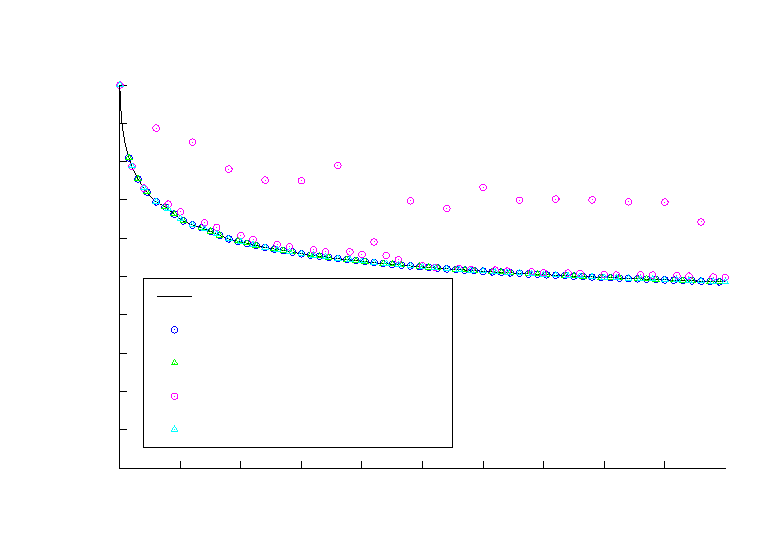
\includegraphics{dmat2_scale}}%
    \gplfronttext
  \end{picture}%
\endgroup
